% PLEASE FOLLOW POSTED GUIDELINES!!

% Please see the two LAr CDR 'guidelines' writeboards in basecamp
% at https://lbne-doc.basecamphq.com/projects/4264323/writeboards
% One is for text, the other for images and figures 

% Replace the following when the name of the experiment is decided
\newcommand{\LBNE}{ELBNF}
\newcommand{\COMPARTMENT}{detector section}
\newcommand{\COMPARTMENTS}{detector sections}

%%%%%%%%%%%%%%%%%%%%%%%%%%%%%%%%%%%%%%%%%%%%%%%%%%%%%%%%%%%%%%%%%%%%%%%%
%%%%%%%%%%%%%%%%%%%%%%%%%%%%%%%%%%%%%%%%%%%%%%%%%%%%%%%%%%%%%%%%%%%%%%%%
\chapter{Data Acquisition}
\label{ch:trig}

The data acquisiton (DAQ) subsystem provides the data collection
in a robust fashion and optimised for the specific needs of the neutrino and
underground physics of the experiment.  The scope includes design,
procurement, fabrication, testing, delivery and installation of a
combination of custom and commerical electronics modules, (including
commodity computing and networking hardware), as well as both
commercial and internally developed software.

The \LBNE\ DAQ must collect data from (a) interactions which are associated
with the beam, (b) high energy ($>100$~MeV) interactions which are asynchronous such as
atmospheric neutrinos, proton decay, cosmic ray muons etc., and (c) low
energy interactions such as those from difuse supernova neutrinos or a
possible supernova explosion in our galaxy.  In the latter case, it is
essential to have the maximum possible uptime, to be sure data is
being collected when a supernova occurs, and to have a sensitive time
of at least 10 seconds, the estimated time a neutrino burst will last,
implemented in ring buffer disk storage.  The design follows many of
the principles of other neutrino and collider experiments with scope
for a multi-level trigger and continuous readout to cope with events,
such as atmospheric neutrinos, that are asynchronous with the beam.

An innovation of the \LBNE\ DAQ is a thin loose coupled upper layer,
as described in section~\ref{sec:daq_upper}, which extends the
modularity of the \LBNE\ far detector design and facilitates both
staging and a possible distributed (worldwide) approach to design and
procurement.   It allows the different \COMPARTMENTS\ to be
operated independently, and in so doing allows an added degree of
robustness to data collection, in particular supernova burst
detection, by giving a method for eliminating entirely even short
periods when the entire detector is off.  It also allows for unique 
design features to be possible in the different \COMPARTMENTS\ 
of \LBNE.

The majority of this chapter describes the full conceptual design for
the main data acquisition which could be used in all, or just some of
the \COMPARTMENTS\ of the experiment.  This is the reference design,
used in the 2015 cost and schedule estimations for \LBNE.  

%% Remove the following to keep it crisp
%There is scope for modification and improvements to this conceptual
%design, however we believe that the one presented here satisfies the
%requirements for the experiment and so gives a realistic indication
%that it is feasible and of the cost.  Further innovation to increase
%robustness or performance is welcome, and the thin layer allows for
%sufficient modularity that innovations can also be added to the later
%\COMPARTMENTS\ after the initial \COMPARTMENTS\ are deployed.

The main data acquisition is introduced in
section~\ref{sec:daq_intro}.  It is comprised of a readout for the
LArTPC based on COB modules (section~\ref{sec:daq_cob}), a readout for
the photon detectors based on SSP modules (section~\ref{sec:daq_ssp}),
a time synchronisation system (section~\ref{sec:daq_time}) and a
readout and trigger generator for auxilliary signals associated with
the experiment (section~\ref{sec:daq_penn}).  The real time data
collection is performed by a toolkit called artDAQ
(section~\ref{sec:daq_artDAQ}) that will implement two arms of data
collection, event-building and processing; the first will stream the
zero-suppressed hits continuously into a trigger processing farm to
locate the positions and times of the interesting detector
interactions and for data storage for supernova studies; the second
arm receives non-zero suppressed data from the times and positions
indentified in the first arm to allow the full data to be collected
for these interesting events.  The run control
(section~\ref{sec:daq_runcontrol}), online monitoring
(section~\ref{sec:daq_om}), slow control
(section~\ref{sec:daq_slowcontrol}) and infrastructure for the DAQ
subsystem (section~\ref{sec:daq_infrastructure}) are also described.
There follows the description of the modular thin upper-layer approach
as introduced above, in section~\ref{sec:daq_upper}.  This allows a
heterogeneous approach to different \COMPARTMENTS\ of the DAQ and
gives the ability to keep the majority of the detector running when
one part needs to stop data taking for maintenance.

\begin{editornote} 
\begin{center}
{\bf Under construction by Giles: New stuff added, old stuff remains}
\end{center}
Add bit about supernova storage and triggereing
\end{editornote}

\section{Introduction}
\label{sec:daq_intro}

\subsection{System overview}

The DAQ subsystem will perform the primary functions of:

\begin{itemize}
  \item Readout of raw data from the LArTPC electronics and the photon
    detector subsystem,

  \item Continuous filtering and assembly of data to be treated
    offline as individual events, including receiving and using the
    Fermilab beam-spill signal, 

  \item Logging data to persistent storage media,

  \item Configuration, online calibration/checkout, and control of 
        operations of detector electronics, including the generation 
        and distribution of timing and control signals,

  \item Control of, and readout of data from, devices 
        providing real-time information on detector, subsystem 
        and environmental conditions, and  

  \item Providing user/operator interfaces for these functions via 
        a run control system.
\end{itemize}

A reference design for the DAQ subsystem is presented in this chapter.
The development of this design is guided by recent experience gained
in the development of relevant systems for the MINOS,
NO$\nu$A~\cite{novatdr} and MicroBooNE~\cite{microboonecdr}
experiments, as well as from experiments with comparable channel
counts and/or experimental conditions, such as D-Zero, CDF, NA48 and
ICARUS.  Guidance and experience is also available from the design and
operation of the LBNE 35t prototype and the futute CERN testing
program.

The DAQ subsystem is to be located external to the cryostat vessel,
with components in the detector halls and in an on-site control
room\todo{It is not yet decided whether there is a computer room underground}.
The interfaces are with the front-end electronics for the LArTPC and
photon-detector subsystems.  To increase robustness and up-time, there
is a comparitively loose coupling between the DAQ subsystems in each
detector hall, to allow calibration or maintenence to proceed in one,
while data collection continues in the others.  The DAQ subsystem
interfaces with the Fermilab Accelerator complex (the beam-spill
signal), and has a read-only interface with the cryogenics subsystem
for logging of conditions.  

\begin{cdrfigure}[DAQ subsystem block diagram]{daq15_main}{Block diagram layout of the main
    components of the DAQ subsystem.}
\begin{tikzpicture}[
  every matrix/.style={ampersand replacement=\&,column sep=0.4cm,row sep=0.6cm},
  to/.style={->,>=stealth',shorten >=1pt,semithick,font=\sffamily\footnotesize},
  data/.style={thick},
%  box/.style={draw,thick,rounded corners,fill=yellow!20,inner sep=.3cm},
  box/.style={draw,inner sep=.1cm},
  boxa/.style={box,align=center}]

% Lay the nodes out using a matrix
  \matrix{   
% 1st row
  \node[boxa] (ce) {Cold\\Electronics};
 \&
 \& \node[boxa] (rce) {RCE\\LArTPC data\\processors};
 \&
 \& \node[boxa] (trigfe) {Trigger\\frontend\\Computers};
 \& \node[boxa] (trigbe) {Trigger\\backend\\Computers}; \\

% 2nd row
 \& \node[box,inner sep=0.4cm] (fthru) {}; 
 \& \node[boxa] (time) {Time\\Sync};
 \&
 \& \node[boxa] (sc) {Slow\\Control};
 \& \\

% 3rd row
  \node[boxa] (pd) {Photon\\Detectors};
 \&
 \& \node[boxa] (ssp) {SSP\\Photodetector\\digitizers};
 \&
 \& \node[boxa] (datafe) {Data\\frontend\\Computers};
 \& \node[boxa] (databe) {Data\\backend\\Computers}; \\
 };

\coordinate (fthruWL) at ($ (fthru.south west)!0.3!(fthru.north west) $);   % West Low edge of fthru 
\coordinate (fthruWH) at ($ (fthru.south west)!0.7!(fthru.north west) $);   % West High edge of fthru 
\coordinate (fthruEL) at ($ (fthru.south east)!0.3!(fthru.north east) $);   % East Low edge of fthru 
\coordinate (fthruEH) at ($ (fthru.south east)!0.7!(fthru.north east) $);   % East High edge of fthru 

\coordinate (trigfeWL) at ($ (trigfe.south west)!0.3!(trigfe.north west) $);   % West Low edge of trigfe 
\coordinate (trigfeWH) at ($ (trigfe.south west)!0.7!(trigfe.north west) $);   % West High edge of trigfe
\coordinate (datafeWL) at ($ (datafe.south west)!0.3!(datafe.north west) $);   % West Low edge of datafe
\coordinate (datafeWH) at ($ (datafe.south west)!0.6!(datafe.north west) $);   % West High edge of datafe

\coordinate (rceEL) at ($ (rce.south east)!0.3!(rce.north east) $);  % East low edge of RCE 
\coordinate (rceEH) at ($ (rce.south east)!0.7!(rce.north east) $);
\coordinate (sspEL) at ($ (ssp.south east)!0.3!(ssp.north east) $);  % East low edge of SSP
\coordinate (sspEH) at ($ (ssp.south east)!0.8!(ssp.north east) $);

\coordinate (rceSR) at ($ (rce.south)+(0.7cm,0) $);  % South right edge of RCE 
\coordinate (sspNR) at ($ (ssp.north)+(0.7cm,0) $);  % North right edge of RCE 
\coordinate (scWL) at ($ (sc.south west)!0.3!(sc.north west) $);  % West low edge of SC 
\coordinate (scWH) at ($ (sc.south west)!0.7!(sc.north west) $);  % West high edge of SC 

\draw[data] (ce) -| ($(fthruWH)-(0.1cm,0)$) -- (fthruWH);
\draw[data] (pd) -| ($(fthruWL)-(0.1cm,0)$) -- (fthruWL);
\draw[data] (fthruEH) -- ($(fthruEH)+(0.1cm,0)$) |- (rce);
\draw[data] (fthruEL) -- ($(fthruEL)+(0.1cm,0)$) |- (ssp);

\draw[data] (rceEH) -- ($ (rceEH)+(0.5cm,0) $) |- (trigfeWH); 
\draw[data] (rceEL) -- ($ (rceEL)+(0.5cm,0) $) |- (datafeWH); 
\draw[data] (sspEH) -- ($ (sspEH)+(0.55cm,0) $) |- (trigfeWL); 
\draw[data] (sspEL) -- ($ (sspEL)+(0.55cm,0) $) |- (datafeWL); 

\draw[data] (trigfe) -- (trigbe);
\draw[data] (datafe) -- (databe);

\draw[data,dashed] (time) -- (rce);
\draw[data,dashed] (time) -- (ssp);

\draw[data,dashed] (scWH) -| (rceSR);
\draw[data,dashed] (scWL) -| (sspNR);

\draw[data,dotted] (fthru.north) -- ($(fthru.north)+(0,2.7cm)$) node [left] {In cryostat} node [right] {Room temp.};
\draw[data,dotted] (fthru.south) -- ($(fthru.south)-(0,2.7cm)$);

\end{tikzpicture}
\end{cdrfigure}
The DAQ subsystem reference design described in this chapter is shown
in figure~\ref{fig:daq15_main} and consists of the following
components:
\begin{itemize}
  \item Logic and processing elements called ``Reconfigurable cluster
    elements'' (RCE) residing on daughter cards in ATCA crates located
    in the detector hall to receive data from the LArTPC.  These carry
    out data merging, buffering and compression and transmission to the
    local frms of commodity computers (see section~\ref{sec:daq_cob})
  \item custom `SSP photon detector digitizers' which digitize and
    process the light signals (described in section~\ref{sec:daq_ssp}) 
  \item two local farms of commodity computers providing two separate
    branches of readout, triggering, event processing and logging of the
    detector computers; these use the artDAQ toolkit for data
    acquisition systems (see section~\ref{sec:daq_artDAQ})
  \item a custom timing system consisting of a master unit, situated
    on the surface, that locks onto a GPS clock and distributes timing
    signals to the data concentrator modules via slave units (see
    section~\ref{sec:daq_time})
  \item dedicated computer nodes that host run control online
    monitoring, database services and slow controls processes
\end{itemize}
%
The DAQ subsystem does not include power-supply hardware for the
LArTPC or front-end electronics, nor does it include the cryogenics
subsystem process-control and monitoring functions.  The SSP readout
modules for the photon subsystem is in the photon subsystem part of
the project.

\subsection{Physics Considerations}

The physics considerations determine the scale of the primary tasks of
digitizing the LArTPC data readout, merging the photon system data,
event building and online processing.  In addition to rates for
processes of interest, the DAQ subsystem design depends critically on
the specifications for the LArTPC and front-end electronics systems,
chosen to satisfy the \LBNE\ physics requirements.  The sampling rate
of 2~MHz has been chosen so as to achieve the required position
resolution along the ionization drift direction. Obtaining sensitivity
to signals that occur independently of the \LBNE\ beam spill, such as
those from nucleon decay, atmospheric neutrinos or supernova-neutrino
bursts, requires a free-running transmission of data from the LArTPC
front-end electronics.  In principle, this same technique can be used
to collect the beam events as well, however we will supplemement the
robustness of the beam data collection by transferring knowledge of
the spill times from Fermilab to the far detector site using GPS.

The task of data transfer is facilitated by multiplexing and utilizing
high-speed data lines (1Gbps) in front-end ASICs in the LAr, and by
redundant \todo{Can we still say redundant? - wording is from the first CDR} data lines that
provide connection to data-acquisition hardware located outside the
cryostat.  The hardware receiving the raw TPC data then perform
zero-suppression and/or data compression, as desired.  A challenge in
real-time is to use the information of the channels which have hits on
them in a particular interaction to determine a larger set of
channels, which including the surrounding ones, that should be read
out.  The design, as depicted in figure~\ref{fig:daq15_main},
addresses this difficulty by using two data paths.  The trigger data
path continuously receives the data from the channels that the online
hardware determines have hits on them.  This determines whenever an
event occurs and designates regions of interest which are to be read
out in more detail.  Ring buffers in the RCEs store the non-zero
suppressed data until the region of interest information is received,
at which point they transmit non-zero suppressed data to the second
path, the Data path which reads out the interesting events (all
candidates of cosmic rays, beam events, atmospheric neutrinos, proton
decays etc.) for all channels within active APAs with no zero
suppression within the entire event drift window period.  This allows
the maximum available information for these, the most important \LBNE\
events, to be recorded for offline analysis using e.g.\ Fourrier
transform deconvolution techniques.

The trigger data path handles all the zero suppressed data and can
store it for long periods, either in ${\cal O}(\mathrm{hours})$-long
ring buffers or in permanent offline storage for collection of data
from a supernova neutrino burst.  Experience from MicroBooNE, which
has a similar division of lossy-compressed and lossless-compressed
data readout, will be vital in optimising this feature of the data
acquisition.  During a supernova neutrino burst, the data path may
also be used for data collection, the optimum way for utilising this
is still to be studied.

In addition to physics considerations, the DAQ design goals include
minimizing the impact of single-point failures, maximizing the uptime
and maximizing the use of commercial components.  The robustness is
addressed in part by some redundancy (and ability to cross-check)
between the two arms of data transfer shown in
figure~\ref{fig:daq15_main}, and by the separation of sub-system
control in different \COMPARTMENTS\ of the experiment
(section~\ref{sec:daq_upper}).

The requirements on the DAQ system are listed in the requirements
documentation~\cite{lar-fd-req}. \todo{Can we remove this, the Rs are
  not so up to date?}

\subsection{Event Rates and Timing}
\label{sec:v5-daq-assumptions}

For the reference design described here, sited at the 4850L of the Sanford Laboratory, the 
atmospheric-muon rate is small enough -- 0.1~Hz within the full LAr-FD active 
volume -- to contribute only negligibly to the DAQ bandwidth requirement.
%For reference, the rate at the alternate 800L site 
%is estimated to be 500~Hz within the active volume.  
%This and other assumptions are discussed below in 
%Section~\ref{sec:v5-daq-assumptions}.  

%The DAQ subsystem design depends on assumptions pertaining to physics goals as well as detector configuration and conditions. 

Signals associated with beam events will be localized within the
LArTPC and synchronous with discrete (${\cal O} (1\,s)$ rep rate)
beam-spill intervals spanning approximately $10\,\mu s$ and will take
${\cal O} (2\,ms)$ for the ionization drifting in the LArTPC to take place.
However other physics events of interest will occur at random times,
and can be dispersed throughout the TPC volume as in the case of
neutrino bursts from supernovae.  Other specific signatures, such as
very slow-moving magnetic monopoles ($\beta < 10^{-3}$) may involve
signals spanning sample times exceeding the ionization-drift time.

Cosmic-ray muons dominate the physics rate, even at the proposed 4850L
site.  However, this rate is negligible with respect to noise sources.
The reference design proposed here would be capable of operation at
shallower depths, up to about the 800L, without sgnificantly impacting
the design.

As described earlier in this report (see
Figure~\ref{fig:tpc-elec-schematic}), the cold electronics for a
single Anode Plane Assembly will consist of twenty \todo{update} 128-channel
Front-End Readout Boards, each providing four digital inputs to the
RCEs.  The Front-End Boards will generate non-zero-suppressed data,
i.e.\ a constant data rate of (1.5 bytes/sample $\times$ 32 wires/link
$\times 2 \times 10^6$ samples/wire/s $=$) 96\,MB/s.

For cosmic-ray muons, the rejection factor is estimated to be $\sim 200$.  
The rejection factor is of course much higher in APAs 
not containing any portion of a physics event.  Radioactive decay 
from $^{39}$Ar and $^{85}$Kr in the LAr, and to a lesser extent from 
detector materials (U/Th/Co/K), is estimated to provide a
65-kHz/APA rate of activity of energy above about 300~keV (0.3 MIPs) 
but less than $\sim 5\,$MeV, while 
electronics noise (assuming 10:1 S/N for 1 MIP, and a threshold of 0.3 MIPs) 
will contribute a relatively low rate per APA of singles.  
Table~\ref{tab:daq-signal-rates} provides a summary of these rate 
estimates.  Work is ongoing to further refine them.
%
\begin{cdrtable}[Rates and data sizes/rates for various processes.]
  {lcccc}{daq-signal-rates} {Per-APA estimates of rates and
    data sizes/rates for various processes.  Mbps denotes millions of
    {\it bits} per second.  Unless otherwise stated,
    estimated numbers of samples and data rates assume suppression of
    signals below 0.3 MIP.  `Inst.\ Data Rate' refers to the number of
    bits in a 2.3-ms long data block divided by this time interval,
    while `Avg.\ Data Rate' factors in the process rate.  A 12-bit ADC
    is assumed, and no allowance is made for data items such as
    time-stamp, etc.}
  
    {\bf Process} & {\bf Rate } & {\bf Samples}
                  & {\bf Inst.\ Data } & {\bf Avg.\ Data}  
                  \cr 
                  & {\bf (kHz/APA)}  & {\bf (per APA)}
                  & {\bf Rate (Mbps)} & {\bf Rate (Mbps)} \cr \hline
    Generic 2.3 ms interval 
                  & 0.43 & $1.06 \times 10^7$ 
                  & 55,000 & 55,000 
                  \cr 
                  (not zero-suppressed) & & & & \cr \hline
    Cosmic ray muons (4850L)
                  &  $6\times 10^{-7}$ & $5 \times 10^4$ 
                  &  260 & $1\times 10^{-4}$
                  \cr 
                  & & & & \cr \hline
%    Cosmic ray muons (800L)
%                  &  0.0034 & $5 \times 10^4$ 
%                  &  260 & 2.0 
%                  \cr 
%                  & & & & \cr \hline
    10 GeV EM shower 
                  &  --- & $1 \times 10^6$
                  & 5,200  & --- 
                  \cr
                  & & & & \cr \hline
    Radioactivity: $\gamma$: U/Th
                  & $\sim 1$ & 40
                  & 0.48  & 0.48
                  \cr
    \phantom{Radioactivity:} $\beta$: $^{39}$Ar, $^{85}$Kr
                  & 63 & 24
                  & 18  & 18
                  \cr
%                  & & & &  \cr 
                  \hline
    Electronics noise
                  & $\sim 1$ & 15 
                  & 0.2  & 0.2 
                  \cr 
                  (not common mode) & & & & \cr \hline
\end{cdrtable}

The conclusion from table~\ref{tab:daq-signal-rates} is that the
average data rates out of the front-end electronics system are
manageable: about 20 Mbps of `salt and pepper' per APA due to
radionuclides in the Ar and LArTPC materials.  Large beam- or
atmospheric-neutrino interactions or showering ultra-high-energy
cosmic-ray muons will result in high (Gbps-level) instantaneous rates
on the scale of the maximum ionization drift period, but contribute
negligibly to the average rate.

\subsection{Architecture Summary}
\label{sec:v5-trig-daq}

The reference design of the DAQ system is summarized in block diagram
form in Figure~\ref{fig:daq15_main}.  Component counts are given in
Table~\ref{tab:daq15_component_counts}. \todo{Update table.  Be
  precise and for what sized detector.}

\begin{cdrtable}[DAQ subsystem component counts]{ll}{daq15_component_counts}
  {DAQ subsystem component counts for one 20-kton module/cryostat.}
    {\bf Quantity} & {\bf Description} \\
   60  &  COBs (Cluster on Board) each with 8 RCEs\\
   20  & 2-slot ATCA Shelves  \\
   2   & Ethernet Switches   \\  
   60  &  TPC Readout Compute Nodes \\
   1   &  Master Timing Unit with GPS Receiver\\
   10  &  Slave Timing Units  (assuming we build new, improved ones) \\
   8   &  Event Builder Compute Nodes  (???) \\
   8   &  Software Filter Compute Nodes (???) \\
   1   &  Run Control Compute Node   \\
   1   &  Slow Control Compute Node   \\
   1   & DAQ Database  Compute Node   \\
\end{cdrtable}

%%%%%%%%%%%%%%%%%%%%%%%%%%%%%%%%%%%%%%%%%%%%%%%%%%%%%%%%%%%%%%%%%%%%%%%%
%%%%%%%%%%%%%%%%%%%%%%%%%%%%%%%%%%%%%%%%%%%%%%%%%%%%%%%%%%%%%%%%%%%%%%%%
\section{COB - Cluster on board modules}
\label{sec:daq_cob}

The primary interface between the TPC front-end electronics (FE) and
the DAQ subsystem consists of an ATCA-based system of RCEs
(Reconfigurable Cluster Elements).  The RCE system receives the
serialized raw data for the FE, performs zero-suppression on it, and
packetizes and transmits the resulting sparsified data to a back-end
data farm for event building and further processing.  Additionally,
the RCE system transmits timing and control signals to the FE as well
as forwarding configuration data to them at start-up.

\begin{figure}[hbt]
  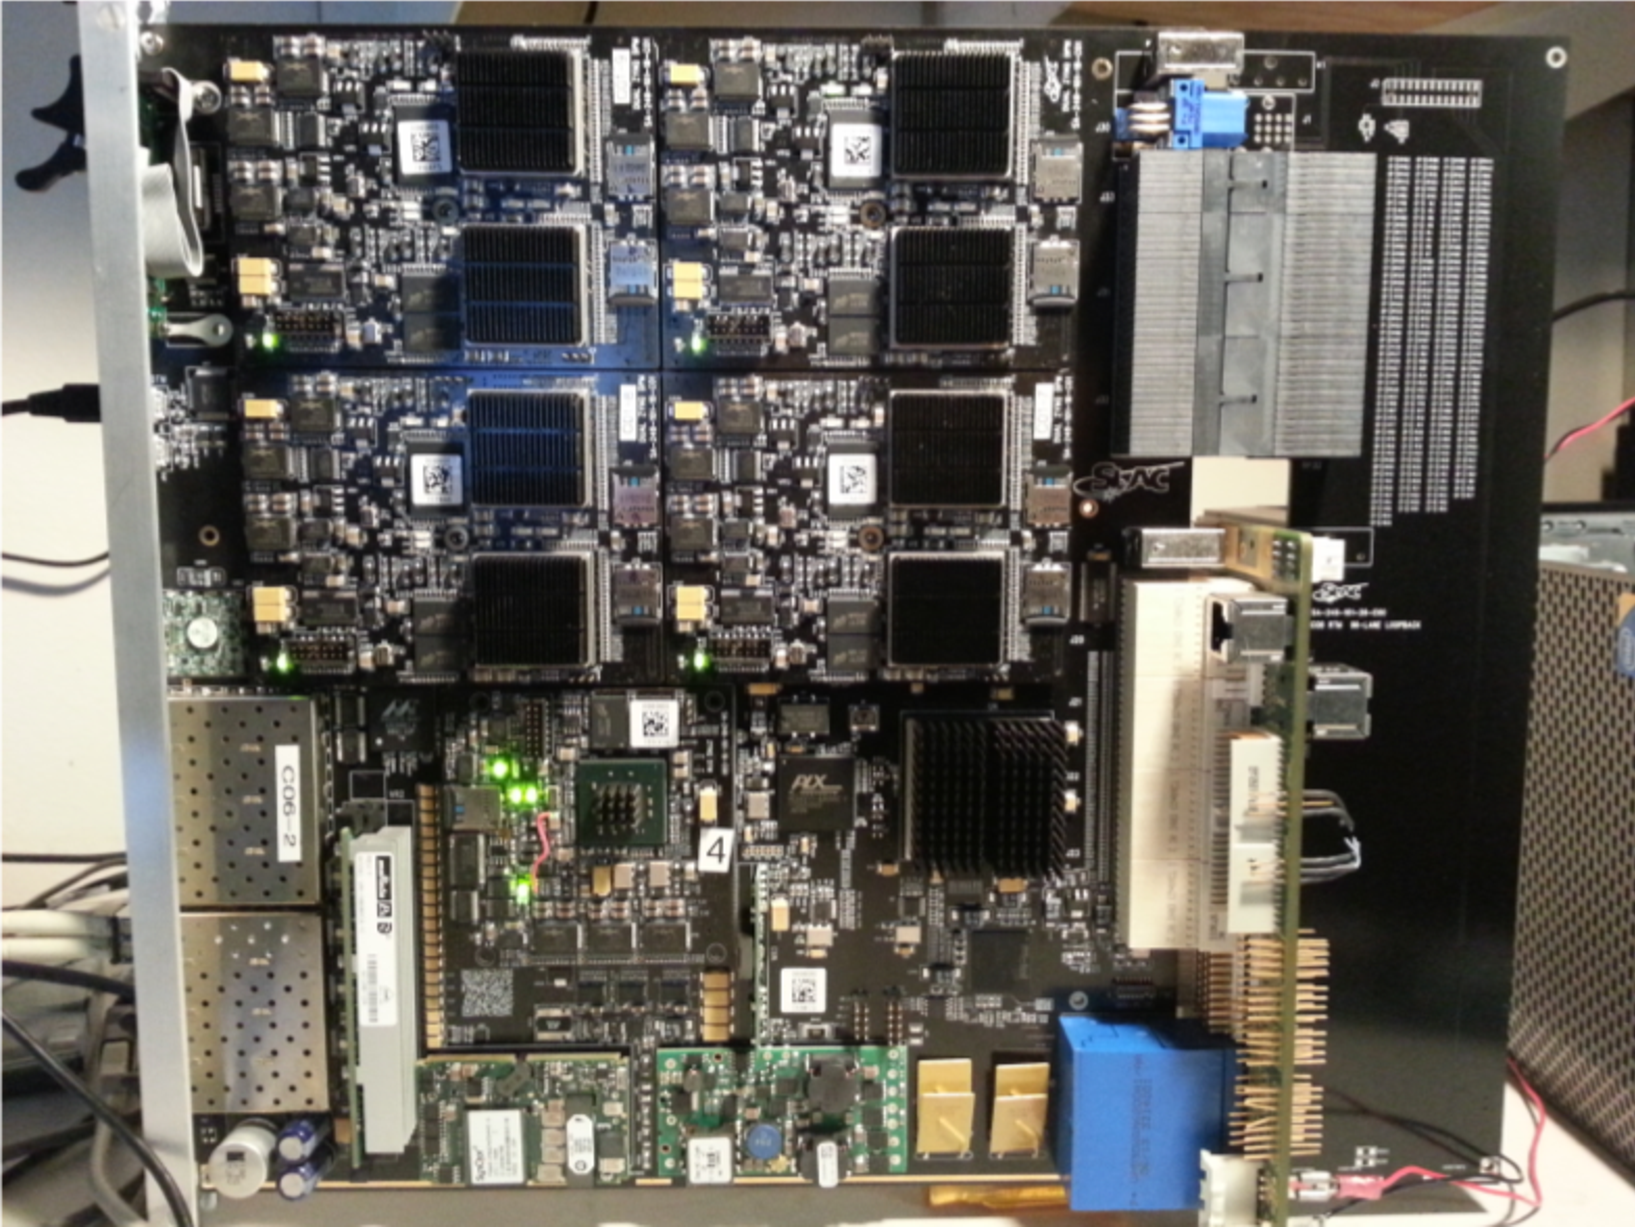
\includegraphics[scale=0.5]{daq15_COB-gen3.pdf}
  \caption{\label{fig:daq15_cob} The COB (left) and RTM (right).  }
\end{figure}
The RCE system consists the following components: a commercial ATCA
shelf (2-, 6-, or 14-slot), a Cluster-On-Board (COB) which is the
"front board" in ATCA terms, and a Rear-Transition-Module (RTM) which
is the "rear board".  The COB is a custom board, developed by SLAC,
which holds the processing power of the system.  The COB (see
Figure~\ref{fig:daq15_cob}) consists of 5 bays for holding daughter
boards, an onboard 10-GbE switch, and both 10- and 1-Gb ethernet
connections for communications with the back-end system.  Four of the
daughter-board bays are for Data Processing Modules (DPM), each of
which can hold up to two RCEs.  The RCE is the core procession unit of
the system; it is made up of a modern SoC (currently, the Xilinx
Zynq-7045) with multiple high-speed I/O ports (up to 10-Gbps each) and
external DRAM \todo{Say how much} and flash memory controllers.  The
other bay on the COB contains the Data Transmission Module (DTM) which
is responsible for distributing timing and trigger information to and
between the DPMs.

While the COB hardware is application agnostic, the firmware and
software on the RCE and the RTM board are application specific. The
RTM provides the mechanical and electrical interfaces between the
front-end (or, in our case, the flange electronics) and the back-end,
as well as other external sources such as the timing or trigger
systems.  In the case of \LBNE, we propose \todo{Add another sentence
  or two of detail about the number of signals, what happens inside
  the flange, make it tie in better with the intro to
  section~\ref{sec:daq_time}.} to use fiber optic connections between
the flange and the TPC DAQ using QSFP+ connectors.  Currently, each
RTM can accommodate up to 16 QSFP+ connections.

With the assumption that each cold FE board multiplexes it's 128 wire
channels to 4 outputs at 1-Gbps each, the non-zero suppressed data for
1 APA can be fed into a single COB (containing 8 RCEs).  Each RCE
would receive data from 2 FE boards, perform zero-suppression, and
send the result to the trigger front-end computers.  There would also
be a large DRAM ring buffer to store a non-zero suppressed copy of the
data, which would be read out on request (see
figure~\ref{fig:daq15_main}) to the data front-end computers.

Figure~\ref{fig:daq15_atcapic} shows a COB in a two-slot ATCA shelf.
There are some options regarding the physical distribution of the
shelves.  One option is to have a smaller shelf at each flange port,
each shelf collecting data from the 2- or 4-APAs accommodated by that
port.  Alternatively, the fibers from all APAs could be routed to a
central location into a smaller number of large ATCA-shelves.

\begin{figure}[hbt]
  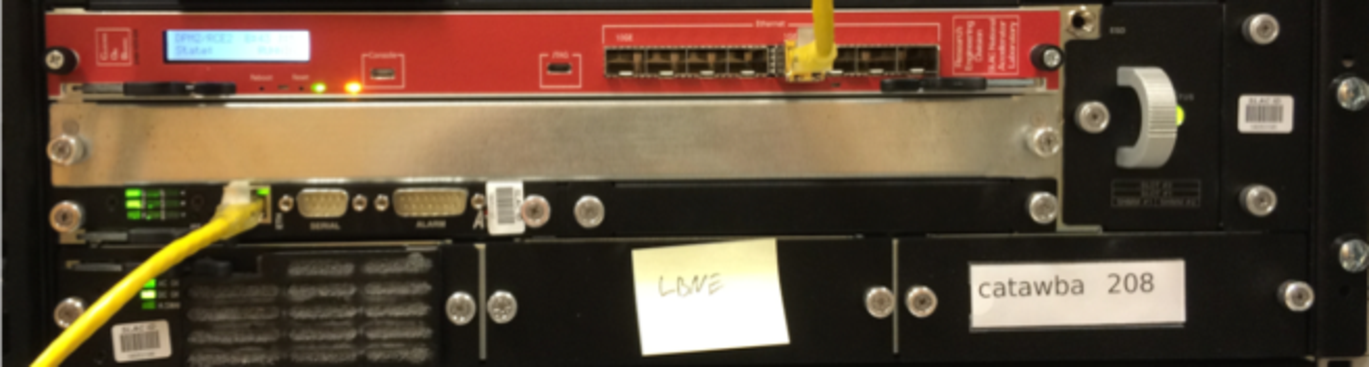
\includegraphics[scale=0.6]{daq15_acta-rtm.pdf}
    \caption{\label{fig:daq15_atcapic}A front view of the ATCA crate with a COB in the top slot. }
\end{figure}

%%%%%%%%%%%%%%%%%%%%%%%%%%%%%%%%%%%%%%%%%%%%%%%%%%%%%%%%%%%%%%%%%%%%%%%%
%%%%%%%%%%%%%%%%%%%%%%%%%%%%%%%%%%%%%%%%%%%%%%%%%%%%%%%%%%%%%%%%%%%%%%%%
\section{Photon detector readout}
\label{sec:daq_ssp}

The photon detection system is digitised and readout by a custom
module called the SIPM signal processor (SSP) which is described in
detail in section~\ref{sec:pd_ssp}\todo{When SSP is in PD chapter,
  refer directly to that instead of this section}\ in the photon detector chapter.
The module has ADC and signal processing hardware.  The output of the
SSP is Ethernet, interfaced with the same Xilinx Zynq architecture as
the COB which is used for the LArTPC data. The SSP therefore is able
to provide control, data and slow-control monitoring independently
from each other which facilitates a consistent interface between the
hardware and software parts of the DAQ.

%%%%%%%%%%%%%%%%%%%%%%%%%%%%%%%%%%%%%%%%%%%%%%%%%%%%%%%%%%%%%%%%%%%%%%%%
%%%%%%%%%%%%%%%%%%%%%%%%%%%%%%%%%%%%%%%%%%%%%%%%%%%%%%%%%%%%%%%%%%%%%%%%
\section{Timing System }
\label{sec:daq_time}

There are comparable requirements of LBNE for timing with the NOvA
experiment.  That experiment uses a Global Positioning System (GPS)
receiver on the surface (in a module called the Master Timing Unit
(MTU) and a protocol that uses four twisted pair connections (on a
standard RJ45 connector) to fan out and then daisy-chain these signals
to the electronics.  We propose using the same concept to the NOvA
timing system, with potential enhancements and modernisation to
distribute the timing from the surface to the underground, among the
readout modules for the photon detector and also for distribution to
the COBs for the LArTPC readout.  In addition, we propose a custom
protocol for synchronisation of the cold electronics boards, which is
fed on the same optical links as described in
section~\ref{sec:daq_rce} from the COBs to the inside of the cryostat.

The timing link is the only physical link other than the
communications network.  Therefore, it must provide several functions.

\begin{itemize}
\item Provide a time stamp so that data can be associated with a
  specific accelerator extraction cycle.
\item Provide a common 64 MHz clock to all front end electronics
  boards.
\item Synchronize the data acquisition system so that all data from a
  given time period is sent to the same event builder.
\item Provide dynamic synchronization to the cold electronics so
  glitches in the clock signal are detected promptly.
\item Enable calibration and test pulses to be generated
  simultaneously for multiple channels.
\end{itemize}

These features are covered in more detail in the sections below.

\subsubsection{Beam triggers and time stamps}

A similar GPS basd system will be used at Fermilab to record the times
of the accelerator spills which generate the 10\,$\mu$s bursts of
neutrinos.  There should be sufficient buffering in the trigger path
of the readout system shown on figure~\ref{fig:daq15_main} so that all
trigger-path data can be buffered while the time stamp of the spill is
sent to the far detector over the internet.  It is likely \todo{Check
  the number of channels, to make this sentence less vague} that by
the time the far detector electronics are constructed, memory is
sufficiently cheap to provide a 0.5\,s-deep ring buffer in the RCE for
the data-path data, in which case the non-zero suppressed data will be
available with the spills.

Since the Fermilab accelerator complex is timed off the 60\,Hz electric
line frequency from the local power company, and the time between
accelerator cycles is a variable number of 60 Hz periods, it may be
possible to predict the time of the spills and avoid the need for such
a long ring buffer.  Experience on MINOS and NOvA have shown that the
variability in the 60\,Hz is too great to accurately predict the
arrival time of a future burst of neutrinos, however \LBNE\ has a
considerably longer readout window (several drift times), and so it
could work for \LBNE.

We have chosen a 64 bit time stamp for the 64\,MHz clock so that all
detector and accelerator data will have a unique time for a 20 year
run of the experiment.  This will allow correlation with non
accelerator physics events such as supernovas as well as such things
as equipment failures.

\subsubsection{Front end clock}

The \LBNE\ detector has very low noise front end amplifiers.  The APA system
is connected to 7\,meter long wires so noise pick up from the clock is
a large concern.  One way to nearly eliminate this noise is to select
a clock frequency that is well outside the bandwidth of the front end
electronics.  This has proven to be a very effective in several other
experiments.  We have chosen 64\,MHz for this design.  The internal
capacitance of the SiPMs in the photon system limits the useful
frequency range \todo{say if it limits from above or below} to about 30\,MHz.  Thus, we can place a double pole (6\,db/octave) filter in front of the digitizers. This reduces any noise
from the clock system by 12\,db.  The SiPM's have large internal gain
so 12\,db coupled with careful cable design should be adequate to
eliminate any possible clock noise.

The wire chamber front end amplifiers digitize at 2\,MHz.  The Nyqvist
frequency is 1 MHz so a 4 MHz single pole filter is quite adequate.
Any noise form the clock system is then suppressed by 48\,db which
should be adequate for this system.

\subsubsection{Time stamping and synchronization}

The data is time stamped by the front end digitizing electronics for
the photon system and the warm receiver electronics for the APA
system.  The location of these systems is flexible but the cost of
cabling will likely constrain the location to be near the feed through
port that contains the cables to the cold electronics.

There will be a master clock system on the surface with will receive
the GPS signals and send a 64 MHz clock over fiber optics to the warm
front end electronics. There will also be two additional lines to each
front end for synchronization and digital data.  Since there are many
front ends, there will be several layers of intermediate drivers to
fan out these signals.

The clock system will operate in a manner similar to the one for the
NOvA experiment.  The master will be loaded over the ethernet link
with a time in the future.  The master will send this time over the
digital link to all the front end systems.  The master will then wait
until the down loaded time equals the GPS time.  When they are equal,
it will send a synch pulse over the sync line to each front end.  The
synch pulse causes each front end to load its time stamp register from
the time load register.  The time stamp register then increments on
each 64 MHz cycle.  This register is 64 bits wide and it is appended
to each data packet.

The accelerator system has a similar master and it can be loaded in
the same way over the internet.  The accelerator start of extraction
is time stamped in an identical manner to the data time stamp and sent
over the internet to the far detector.

The detector is nearly a mile underground so there is a significant
delay between the detector master clock (which is the same as the
accelerator master clock) and the front end electronics.  This delay
is compensated for by measuring the time delay to each front end board
and digitally delaying all the clock signals by the difference between
the delay to a given front end and the longest delay in the system.
The delay is determined automatically by each front end system as
follows.  There is a loop back connector on the data and synch lines
at each front end system.  There is a special mode where a pulse on
the synch line is sent back over the data line.  The fanout that is
driving a given front end can then measure the time between itself and
the front end.  The same system can measure the time delay between
each layer of fan out.  These delay times are then loaded into a
digital delay registers at the fan outs and front ends so all front
ends receive the synch pulse at the same physical time.  The time
stamp registers that are loaded into the front ends are corrected for
this delay so that the time stamps reflect true GPS time.

The data rates at the far detector are low enough that a software
trigger can be used instead of a dedicated hardware trigger.  This
system operates by sending data to a special trigger farm.  This
requires that all the data come from the same physical time period.
The time stamp system easily provides this synchronization.  Each
front end has a ``data enable'' bit that must be set before any data is
recorded.  At initialization, this bit is turned off.  When the synch
signal arrives to load the time stamp register, it also sets the ``data
enable'' bit.  Since this occurs at the same physical time for the
entire detector, it provides the necessary synchronization.  The data
acquisition software need only monitor the ``data enable'' to know when
data taking has started.  It can read the time load register to know
the time that data taking started.

\subsubsection{Dynamic Synchronization}

This detector has several hundred thousand channels of cold digitizers
that are driven by the 64 MHz clock.  All of this data arrives
synchronously at the warm electronics.  It is possible that glitches
on the clock line could put the data stream off by one or more bits
resulting in lost data.  It might be possible to check the data in the
warm electronics but it also possible to resynchronize the ADC’s via
the clock line.  This is done by phase encoding the start of an ADC
conversion cycle on the clock line.  For example, if there are 16
channels on an ADC chip, the clock line would phase encode the start
of a 16 channel conversion cycle.  If the front end was not internally
at the start of a conversion cycle, it would reset its internal clock
and send out an error message.  The warm electronics would also check
the phase encoding to spot failures in the clock distribution system.

\subsubsection{Calibration and test pulses}

Calibration and test pulses need to be sent to the various front ends
so that they all occur at the same physical time.  This can be done by
phase encoding additional signals on the clock line.  The front ends
that are to generate calibration or test pulses are enabled by the
control system.  Then, when they see the test or calibration signal on
the clock line, they generate the appropriate pulse.

\section{Readout of auxilliary signals}
\label{sec:daq_penn}

\todo{Write a bit about the Penn board, how it is useful in 35t and
  CERN test, and that we want to keep it to allow external triggers to
  the cavern to be supported for diagnostics, even though there are
  currently no physics needs identified for them.}

%%%%%%%%%%%%%%%%%%%%%%%%%%%%%%%%%%%%%%%%%%%%%%%%%%%%%%%%%%%%%%%%%%%%%%%%
%%%%%%%%%%%%%%%%%%%%%%%%%%%%%%%%%%%%%%%%%%%%%%%%%%%%%%%%%%%%%%%%%%%%%%%%
\section{Event Building and Triggering}
\label{sec:daq_artDAQ}

The event building and triggering function of the LAr-FD DAQ system 
will be performed by the data-farm computers.  Event data will be staged 
locally before being transmitted in quasi real-time (nominally to Fermilab) 
for archival to persistent storage. 

\subsection{Artdaq}

The data acquisition software for the 35-ton prototype detector is
based on artdaq which is a toolkit for building DAQ systems.  It has
been developed at Fermilab and is in use in several other experiments.
Within artdaq, core DAQ functions are provided by the toolkit, and
experimenters develop the modules that perform the functions that are
specific to the experiment.  For the 35-ton detector, LBNE
collaborators have developed modules that configure and read out the
COB and SSP boards that are connected to the LArTPC and photon system
detectors, respectively.  Members of the experiment are also
developing reconstruction and filtering software modules that will
analyze the data as it is acquired.  The artdaq-based DAQ system for
the 35-ton detector has been successfully used to acquire data in
electronics and detector integration tests, and artdaq has been the
default choice for the DAQ framework for the full LBNE detector for
some time.  As part of this, a preliminary design has been developed
for the full detector to use a two-stage artdaq system to stream
zero-suppressed data into a farm of processes, run software modules to
find events of interest, and use the results of this software trigger
to initiate the readout of all of the data produced for the events of
interest.

In thinking about the data acquisition system for a reconfigured
long-baseline neutrino experiment, it is recognized that using a
toolkit such as artdaq has advantages in that it allows experimenters
to leverage existing infrastructure and only develop the components
that are necessary for their experiment.  In addition, there are
advantages to using the same event analysis framework online and
offline (artdaq uses art).  This allows experimenters to develop and
substantially test their software in an offline environment and only
include the full DAQ infrastructure for final testing.

\subsection{Event Building}

At present it is imagined that an event will consist of raw data from the 
entire detector, spanning a time interval yet to be determined.  To construct 
such an event, DCM packets corresponding to data with a common (range of) 
timestamp value(s) will be routed to a particular data-farm node.  

An alternate scenario considers events as being localized to individual 
APAs, or possibly small APA clusters.  Individual farm nodes would work 
only on the corresponding data to generate event records.
This concept is attractive in that (1) the routing of data to farm nodes 
is simplified, and (2) event record sizes are kept as small as possible.  
The main drawbacks are that (1) offline processing/analysis of these event 
records for physics events with activity spanning geographical 
boundaries would become more cumbersome; (2) certain physics studies, such 
as proton-decay searches, might benefit from 
simple access to data-registering activity in remote sections of the detector; and (3) auxiliary data  
would either be unnecessarily duplicated or 
would have to be stored in its own event record, again adding complexity 
to the data-analysis process.  Evaluation of this alternative is ongoing.

\subsection{Event Data Model}

We will need to develop an Event Data Model (EDM).  It may be advantageous 
to implement the raw data EDM in a custom format, as opposed to one based on 
ROOT.  Experience with MicroBooNE will be helpful in optimizing the design 
for this.

\subsection{Triggering and Selection for Output Streams}

Significant work remains to understand how data-farm nodes will carry out 
event filtering and creation of separated physics/task-specific data 
streams.  
%prev phrase a bit confusing AH
Use of the \LBNE\ beam-spill signal to identify events recording 
beam-induced activity is expected to be straightforward.  However, 
identifying events of interest that lack such a signal requires study.  
Is it sufficient to find a suitable way to generically veto events based 
on lack of coherent detector activity, or must `positive' signatures for 
each of the physics processes of interest be identified for triggering?  
To indicate the range of signatures, 
these processes of interest include, for example, (1) beam-induced events 
for which the corresponding beam-spill signal is missing due to 
network failure or other malfunction, (2) atmospheric-neutrino interactions, 
(3) supernova-neutrino bursts, (4) proton decay, and (5) magnetic-monopole 
incidence.  

\subsubsection{Rejection of Event Records}

Since the dominant rate is due to dispersed low-energy activity 
associated with radionuclide decays, simple trigger primitives can be 
generated and combined so as to reject event records failing well-defined 
(and easy-to-model) criteria.  
For example, event records in which no APAs 
register energy deposition in excess of some threshold (say 5~MeV) 
will be sufficient to reject most background events.

\subsubsection{Event selection for Physics-Specific Streams}

Even given the above statements about event rejection, it is desired to 
perform some type of high-level event reconstruction to identify candidates 
compatible with specific physics signatures.  This level of analyses is 
essential both for online detector performance diagnostics as well as 
for the case where candidate event records of particular types are to be 
written to parallel output streams.  For the former application, 
an unanticipated shortfall in the DAQ data farm computing capacity 
could be easily addressed through establishment of a separate computer farm 
for online analysis.
For the latter application, it would be necessary to adjust the size of 
the data farm depending on the processing requirements.  These are not 
known at this time.  However, with anticipated costs for commodity 
computing systems, it is not expected that the overall cost of the 
DAQ/online computing systems would increase significantly relative to 
the currently budgeted system.

%%%%%%%%%%%%%%%%%%%%%%%%%%%%%%%%%%%%%%%%%%%%%%%%%%%%%%%%%%%%%%%%%%%%%%%%
\section{Run Control }
\label{sec:daq_runcontrol}

\todo{Likely remove this first waffle paragraph} The scope of functionality
of the Run Control system includes operation of DAQ subsystem
components, configuration of front-end electronics, control of power
supplies and other auxiliary equipment, and control of data
collection.  Development of a user interface for experimenters during
data-taking and for technical personnel to assist with commissioning
and debugging activities is key.  To date, limited effort has been put
forth in the design of the Run Control system.  To the extent that the
challenges faced are similar to those that have been addressed at
MINOS and ICARUS, no technical obstacles are foreseen.  As the designs
of the DAQ and other subsystems continue to develop, specifications of
the Run Control system will become more concrete.

The LBNE run-control system will be the primary control and monitoring
interface to all data acquisition detector systems for use by detector
operators and other users.  This run control system will provide
several key functions that will make the collections of specific data
acquisition and monitoring systems (referred to as "components")
appear as a single, integrated system with a common control,
monitoring, alert and information display interface.  This common view
of the "system of systems" will ease the training burden on detector
shift operators, allowing for rapid response in the event of system
error conditions.

This design is modeled on the successful IceCube Neutrino Observatory
experiment-control system, known as IceCube
Live\cite{comp:icecube-live}.  The overall design presented here is
simplified, since the geographical and networking constraints for LBNE
are considerably more straightforward than for the extremely remote
South Pole site.

%  IceCube live cite is:
%@inproceedings{comp:icecube-live,
%title = "{Searching for Neutrinos Using Python at the Bottom of the World}",
%author = {K.~S.~Beattie and D.~Glowacki},
%booktitle = {PyCon 2009},
%year = 2009,
%note = {\url{http://us.pycon.org/2009/conference/schedule/event/19/}},
%}

The LBNE run control system features a modular design.  This design,
shown in Figure~\ref{fig:expcont} has a dedicated Run Control server,
which handles the control messages and communication with all
components, GUI and command line front-end control interfaces, and DB
Server to manage recording of reported information in an organized
form.

\begin{figure}[htb]
  \centering
  \begin{center}
    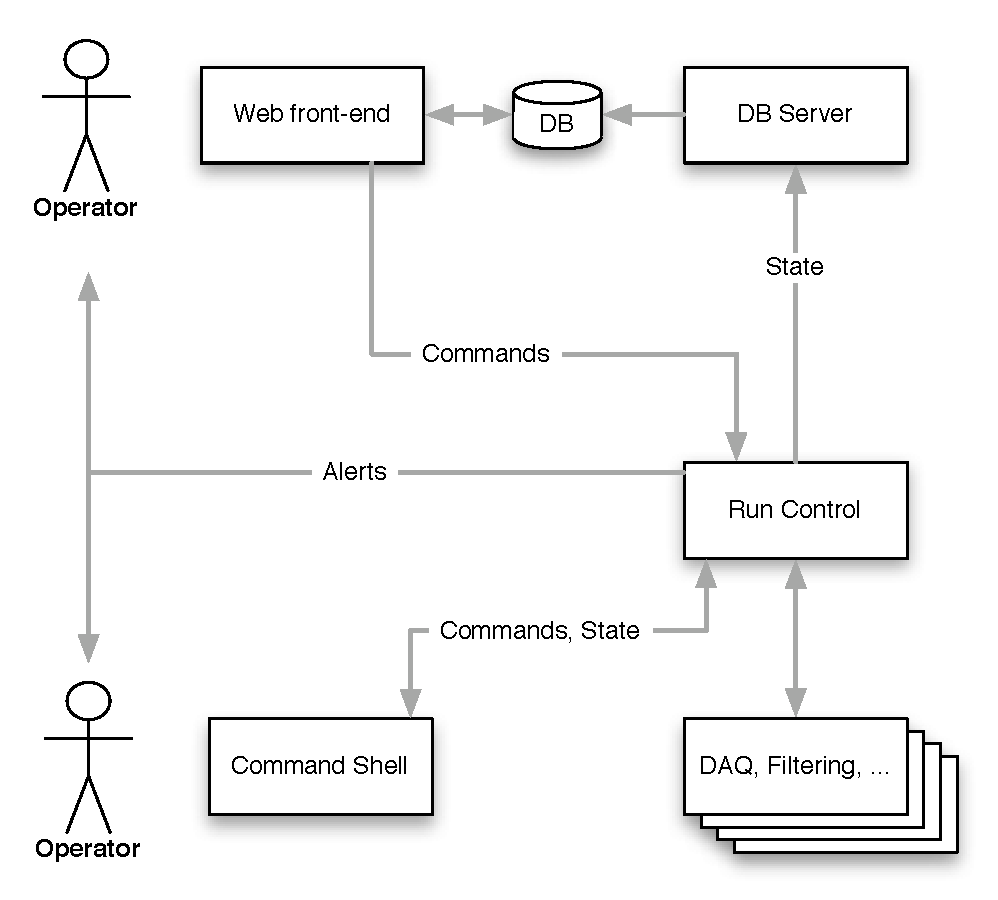
\includegraphics[width=80mm]{RCExpCont}
  \end{center}
    \caption[Run control system]{LBNE run control system design.}
  \label{fig:expcont}
\end{figure}
The LBNE run control system provides several key capabilities, each described below.

\subsubsection{Control and monitoring of LBNE components}
The LBNE run control system will provide a control and monitoring
interface that can be integrated into each component.  This will allow
operators to monitor and change the state (for example: Running,
Stopped, or Error) of each component.  This component control will be
available by both command line interface and graphical user web
interface.  This centralized control of all components that make up
DAQ systems will support complicated dependencies between components,
for example requiring that the DAQ be in a running mode before
starting a calibration system.

\subsubsection{Display of component monitoring and alerts}
During normal operation, all LBNE components will report system
monitoring and health values to the run control system and will be
available for graphical display.  These values can include items such
as overall component health, trigger rates, memory buffer status or
rack temperatures.  These values will be archived in a database and be
presented in a detailed graphical user interface.  This interface can
be customized to the intended audience, with shift operator pages
presenting just high level status information, and expert views that
show detailed, per-channel information for use in detector debugging.

Historical views of component monitoring information will also be
available via the user interface.  This will enable exploration of
historical reported information and correlation analysis between
detector components.  Detector components are not required to be under
LBNE run control state control, but can simply report useful
information.  This type of reporting-only integration could
potentially be useful for offline systems, and would allow the
creation of a more complete historical view of detector history, with
information from data collection displayed side-by-side with
information from offline data analysis.

The LBNE run control system can also generate alerts to detector
operators and/or component experts if reported monitoring information
is outside expected ranges or a system component is in an error state.
These alerts can take any form (email, SMS, etc) and will be a unified
mechanism for alerting operators/experts of operational issues.

\subsubsection{Manage per-run information}
The LBNE run control system will also be responsible for issuing a
unique number to each segment of data collected by data acquisition
systems (commonly referred to as a run number), as well as collecting
all user settings selected for a run.  This information will include
identifiers for configurations used, components selected for operation
during a run, and any provided operator comments.  This information
will be stored in a database, and made available for
collaboration-wide use in online and offline analysis processes.

\subsubsection{Technology}
The LBNE run control system makes use of several standard network and
web technologies.  These include:
\begin{itemize}
\item{XML-RPC - A remote procedure calling library that uses the XML
    formatted messages to issue commands to remote processes, allowing
    the run control server to remotely control components}
\item{JSON - An open standard for message formatting that allows
    arbitrary data to be packaged in a human-readable format using
    name-value pairs for transmission.  Used by the run control system
    components to format and send arbitrary complex monitoring
    records.}
\item{ZeroMQ - A high performance message transport system that allows
    a large number of clients to report information to the run control
    server.}
\item{DJANGO - A graphical web content framework that can easily query
    and display information from DB records.  The run control server
    stores recorded monitoring information in database tables, which
    are available for graphical presentation within the web-base user
    interface.}
\end{itemize}
While these technology choices are selected for their robust designs,
the modular design of the LBNE run control system allows for
flexibility in utilizing other technologies as replacements if that
becomes necessary or is desired.

\section{Online Monitoring}
\label{sec:daq_om}

%%%%%%%%%%%%%%%%%%%%%%%%%%%%%%%%%%%%%%%%%%%%%%%%%%%%%%%%%%%%%%%%%%%%%%%%
%%%%%%%%%%%%%%%%%%%%%%%%%%%%%%%%%%%%%%%%%%%%%%%%%%%%%%%%%%%%%%%%%%%%%%%%
\section{Slow Control Systems }
\label{sec:daq_slowcontrol}

The Slow Control system is a critical element of the DAQ, providing the 
main interface to power supplies for the detector and electronics as well  
as to equipment used to monitor the operational status of the detector and 
supporting systems.  As in the case of the Run Control system, the 
development of the conceptual design for the Slow Control system is in 
its early stages.  Again, based on experience from other experiments, 
no obstacles are foreseen with regard to the development of a robust 
system.

%%%%%%%%%%%%%%%%%%%%%%%%%%%%%%%%%%%%%%%%%%%%%%%%%%%%%%%%%%%%%%%%%%%%%%%%
%%%%%%%%%%%%%%%%%%%%%%%%%%%%%%%%%%%%%%%%%%%%%%%%%%%%%%%%%%%%%%%%%%%%%%%%
\section{DAQ Infrastructure }
\label{sec:daq_infrastructure}

\subsection{Wide Area Network}

As in the case of MINOS and NO$\nu$A, it is expected that event data can be 
transmitted over the network to Fermilab.  Although rates for events of 
interest are comparable, data throughput for the \LBNE\ LArTPC is 
expected to be at least an order of magnitude higher.  A detailed 
analysis of the requirements of Sanford Laboratory for the appropriate level of 
connectivity within and off the lab site will need to be carried out.

\subsection{Online Data Storage}

To protect against signficant periods of absent network connectivity, it 
is desired to store a significant amount of the data emerging from the 
DAQ to local storage.  A local data storage facility of $\sim 100\,$TB is 
expected to be more than adequate for five days worth of detector data, 
even without prescaling cosmic-ray muon events.

\subsection{Power and Cooling}

Power and cooling requirements for the DAQ system described here are 
modest.  DCMs operate at below 50~Watts each, while the maximum power 
consumed by each of the two Cisco 4948Es is 275~Watts.  Assuming 
power supplies that operate at 75\% efficiency, and accounting for 
other components, the total DAQ subsystem budget for power 
in each 20-kton detector/cryostat hall is likely to be below 15~kW.

%%%%%%%%%%%%%%%%%%%%%%%%%%%%%%%%%%%%%%%%%%%%%%%%%%%%%%%%%%%%%%%%%%%%%%%%
%%%%%%%%%%%%%%%%%%%%%%%%%%%%%%%%%%%%%%%%%%%%%%%%%%%%%%%%%%%%%%%%%%%%%%%%
\section{Modular thin upper-layer}
\label{sec:daq_upper}

The thin upper layer of the data acquisition subsystem allows the
\COMPARTMENTS\ of the experiment to have semi-independent and
autonomous data taking --- essentially each \COMPARTMENT\ has sufficient
components (timing system, readout of detectors, data storage and
database storage) to run on its own, including having an independent
run-control state.  The thin upper layer allows the whole detector to
be monitored and controlled as a single big detector, for simplicity
in operation.  It also allows triggers in one \COMPARTMENT\ to initiate
data collection in the other \COMPARTMENTS.

The essential difference between this and having a single data
acquisition for the entire far detector is that if one \COMPARTMENT\
needs maintenance, or if the data collection stops due to a
communication problem or other reason, the other \COMPARTMENTS\ will
continue data collection uninterrupted.  If the complete detector is
not in data taking mode, this will be indicated on the operations
status and alarms screen and the operator will be able restart the
\COMPARTMENT\ and add it back into the overall run.  The run-log
database will indicate the periods when any compartment is missing
from the overall data collection.  It is felt that a mechanism by
which the entire detector does not stop data collection is essential
for a detector with the goal of collecting data from a
once-in-30-years supernova explosion event.  The thin upper layer
concept will also improve overall uptime of the detector.

Each \COMPARTMENT\ runs as a separate data acquisition system with all
the real-time functions being capable of being run independently.
Each compartment has its own run-start and run-stop mechanisms (with a
standardised interface for initiating these commands and obtaining
state status information); its own timing system (required to be
synchronised to UTC to within 10$\mu$s, although it is likely with GPS
that a more stringent limits will be met by the individual
\COMPARTMENTS); its own data storage and data catalogue (with
a standard format for data and for indicating the period of collection
in each file).   Each \COMPARTMENT\ will also have its own independent
storage for slow control measurements.

A centralised `manager' for triggers across the entire detector will
be implemented.  This places a number of requirements on the readout
of the individual \COMPARTMENTS, although note that none of these is
more arduous than that required in order to collect beam spill data on
its own.  The \COMPARTMENTS\ are able to report when the activity it is
detecting warrants triggering of the adjacent (or all) \COMPARTMENTS,
which will be e.g.\ when a cosmic muon, atmospheric or beam neutrino
etc.\ is detected.  These are likely to only occur once every minute,
and a maximum acceptable rate at which a \COMPARTMENT\ should report
will be about one every five seconds.  The reports should arrive at
the central manager within 150\,ms of the event occurring.

The readout in the \COMPARTMENTS\ should be capable of storing the
complete set of signals for at least 200\,ms.  The central manager
will report back to the \COMPARTMENTS\ within this time any requests
from adjacent \COMPARTMENTS\ to collect data within a certain period.
The central manager will also distribute the spill timing from the
Fermilab LBNF beam to the \COMPARTMENTS.  It is likely that the
communication between the \COMPARTMENTS\ and the central manager are
implemented with a dedicated Ethernet network.  The connection setup
will be for the individual \COMPARTMENT\ to subscribe to the central
management service, that way if the central management is not present
or stops, the \COMPARTMENT\ can run independently (although, of course,
it will not receive trigger requests from the other \COMPARTMENTS\ in
this case).  It is possible that an alternative way for a \COMPARTMENT\
to obtain the spill timing information independently of the central
manager may be available.

The run control will consist of a dedicated run-control for each
\COMPARTMENT\ which permits run-starts, -stops, monitoring, logging,
run-mode selection and configuration.  These run-controls can have
functions which vary between \COMPARTMENTS, but will conform to a
standard overall scheme to allow the operator to use a unique
interface (i.e.\ accessible from one web-page) to control and monitor
the entire experiment.  There will be a separate section of the
run-control which will give the overall status of the \COMPARTMENTS\ as
a whole.  It will be regarded as a fault situation unless all
\COMPARTMENTS\ are taking data in production configurations. 

The above parts of the thin upper-layer (the centralised manager and
the ability for the run-control to treat the \COMPARTMENTS\ as
autonomous, with an additional overall status) are all that is needed
in the real-time part of the DAQ subsystem.  A second part of the thin
upper-layer runs offline, shortly after the data collection has been
completed.  This part operates as a batch system on a farm of
computers and combines the data from the individual \COMPARTMENTS\
(which will have data files spanning different periods of time) into
a single sequence of time-ordered files for archival and production
use offline.  The beamline status and monitoring data will be
transferred from Fermilab and incorporated into the files as well
(essentially being regarded as an additional pseudo-\COMPARTMENT).
